\section{partitioning}

In Quicksort, we partition our input into two sets: those smaller than the 
pivot, and those larger or equal. The situation in Quickhull is more similar
to the Dutch National Flag Problem, with the following three options for each
point: belonging in $S_1$, in $S_2$, or neither. The key difference is that
we do not need to preserve the points belonging in neither. This allows us
to modify the more efficient algorithms for bipartitioning.


\subsection{Sequential Partitioning}

Bramas showed in \cite{} that it is possible to vectorize the partitioning
of Quicksort. This is done by reading a vector of values from either the
left or right of the array, partitioning this vector in registers, and
then writing it back to the front and back of the array. During this process,
the invariant of Figure~\ref{fig:invariant_bramas} is maintained.

\begin{figure}[ht]
    \resizebox{\columnwidth}{!}{%
        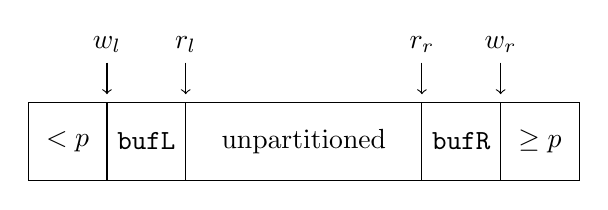
\begin{tikzpicture}
            \draw (0, 0) rectangle (1, 1) node[midway] {$< p$};
            \draw (1, 0) rectangle (2, 1) node[midway] {\texttt{bufL}};
            \draw (2, 0) rectangle (5, 1) node[midway] {unpartitioned};
            \draw (5, 0) rectangle (6, 1) node[midway] {\texttt{bufR}};
            \draw (6, 0) rectangle (7, 1) node[midway] {$\geq p$};

            \draw[->] (1, 1.5) node[above] {$w_l$} -- (1, 1.1);
            \draw[->] (2, 1.5) node[above] {$r_l$} -- (2, 1.1);
            \draw[->] (5, 1.5) node[above] {$r_r$} -- (5, 1.1);
            \draw[->] (6, 1.5) node[above] {$w_r$} -- (6, 1.1);
        \end{tikzpicture}
    }
    \caption{Invariant for partitioning an array into values smaller than
             a pivot $p$ and larger or equal than $p$. The values in
             \texttt{bufL}, \texttt{bufR} are buffered and can be safely
             overwritten. A write and a read pointer are maintained for
             the left and right side of the array.}
    \label{fig:invariant_bramas}
\end{figure}

Let $d$ be the number of element fitting in a vector register. The invariant
is started with \texttt{bufL} and \texttt{bufR} having space of at least
$d$ elements. As we read and write $d$ elements per iteration, the sum
of $r_l - w_l$ and $w_r - r_r$ stays $2d$, ensuring that at least one side
has enough space to write $d$ elements to.

There is enough space on the left whenever

\begin{multline}
(r_l - w_l) \geq d \iff r_l - w_l \geq 2d - (r_l - w_l) \\
\iff r_l - w_l \geq w_r - r_r.
\label{eq:bramas}
\end{multline}

In this case there is already enough space on the left, so we take this as
condition to read $d$ elements from the right. Analogously, there is enough
space of the right when this condition does not hold.

Though Bramas uses a specific avx512 instruction to partition the vector,
the authors of \cite{} show that this can be done in a portable manner by using
the Highway library \cite{}.

We use almost the same algorithm: we write points belonging in $S_1$ to the
left, and points in $S_2$ to the right. As we may write back less than
$d$ elements, we get some undefined parts of the array as illustrated in
Figure~\ref{fig:invariant_qhull}.

\begin{figure}[ht]
    \resizebox{\columnwidth}{!}{%
        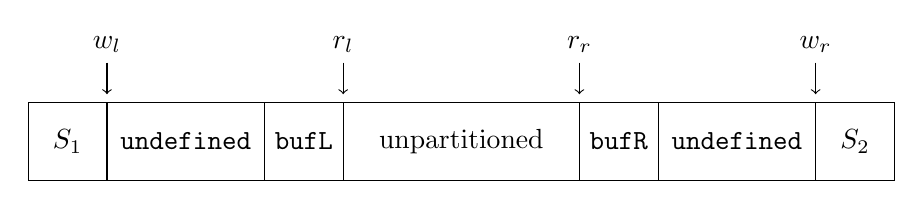
\begin{tikzpicture}
            \draw (0, 0)  rectangle (1, 1)  node[midway] {$S_1$};
            \draw (1, 0)  rectangle (3, 1)  node[midway] {\texttt{undefined}};
            \draw (3, 0)  rectangle (4, 1)  node[midway] {\texttt{bufL}};
            \draw (4, 0)  rectangle (7, 1)  node[midway] {unpartitioned};
            \draw (7, 0)  rectangle (8, 1)  node[midway] {\texttt{bufR}};
            \draw (8, 0)  rectangle (10, 1) node[midway] {\texttt{undefined}};
            \draw (10, 0) rectangle (11, 1) node[midway] {$S_2$};

            \draw[->] (1,  1.5)  node[above] {$w_l$} -- (1,  1.1);
            \draw[->] (4,  1.5)  node[above] {$r_l$} -- (4,  1.1);
            \draw[->] (7,  1.5)  node[above] {$r_r$} -- (7,  1.1);
            \draw[->] (10, 1.5)  node[above] {$w_r$} -- (10, 1.1);
        \end{tikzpicture}
    }
    \caption{Invariant for partitioning a set of points $P$ into 
             $S_1$ and $S_2$ as described in 
             Algorithm~\ref{alg:quickhull_basic}. 
             The values in \texttt{bufL}, \texttt{bufR}
             are buffered and can be safely overwritten. The values marked
             as undefined are not buffered and can be safely overwritten.
             A write and a read pointer are maintained for
             the left and right side of the array.}
    \label{fig:invariant_qhull}
\end{figure}

As $(r_l - w_l) + (w_r - r_r) \geq 2d$, the inequalities of 
Equation~\ref{eq:bramas} hold in our case as well.

\subsection{Parallel Partitioning}

Partitioning has linear complexity, so it is very likely to be limited by
bandwidth. For this reason, minimizing data-movement is the primary design goal
of the parallel algorithm. The algorithm consists out of two conceptual steps:
a parallel step where each thread works on a subset of $P$ local to it, and 
a sequential cleanup step. 

\subsubsection{Local Partition}

We first divide the points over the threads in block-cyclic fashion 
(Figure~\ref{fig:blockcycl}) according to some block parameter $b$.

\begin{figure}[ht]
    \resizebox{\columnwidth}{!}{%
        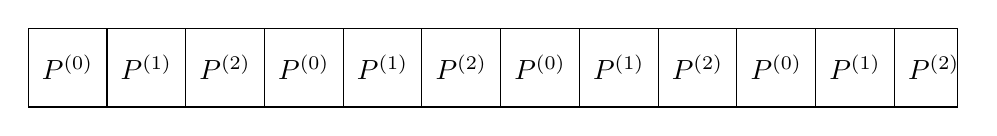
\begin{tikzpicture}
            \foreach \i in {0, ..., 10} {
                \draw (\i, 0) rectangle (\i + 1, 1);
            }
            \draw (11, 0) rectangle (11.8, 1);

            \foreach \i in {0, ..., 3} {
                \node at (3 * \i + 0.5, 0.5) {$P^{(0)}$};
            }
            \foreach \i in {0, ..., 3} {
                \node at (3 * \i + 1.5, 0.5) {$P^{(1)}$};
            }
            \foreach \i in {0, ..., 3} {
                \node at (3 * \i + 2.5, 0.5) {$P^{(2)}$};
            }
        \end{tikzpicture}
    }
    \caption{Block cyclic distribution over $3$ threads. Each square represents
             $b$ elements, except the last one that may contain less.}
    \label{fig:blockcycl}
\end{figure}

To be more precise, given $n$ points total and $n_t$ threads, we partition
the index set $I = [0, n)$ into

$$I^{(t)} = \{t \cdot b + l \cdot n_t \cdot b + j \ | \ 0 \leq j < b,
                0 \leq t \cdot b + l \cdot n_t \cdot b + j < n\}$$

for $t = 0, \cdots, n_t - 1$. Thread $t$ can then work on its subset
$P^{(t)} := \{P[i] \ | \ i \in I^{(t)}\}$ independently from the other threads.

We have each thread partition its $P^{(t)}$ in parallel, returning 
$c_{1}^{(t)}, c_{2}^{(t)} \in I^{(t)}$ such that
$\{P[i] \ | \ i \in I^{(t)}, i < c^{(t)}\} \subseteq S_1$
and $\{P[i] \ | \ i \in I^{(t)}, c^{(t)} \leq i\} \subseteq S_2$.
Denoting $c_{l}^{\min / \max}$ for the minimum / maximum of $c_1$, $c_2$, this
gives us a permuted $P$ where indices in $[0, c_1^{min})$ belong to $S_1$,
indices in $[c_{1}^{\max}, c_2^{\min})$ are in $(S_1 \cup S_2)^c$, and
indices in $[c_2^{\max}, n)$ are in $S_2$, as depicted in 
Figure~\ref{fig:local_part}.

The key observation is that for random $P$ and $n_t, b \ll n$, the ratio 
$|S_1| : |S_2|$ is roughly equal to $|S_1 \cap P^{(t)}| : |S_2 \cap P^{(t)}|$.
This means that the $c_1^{(t)}$s are expected to be close to each other, and
the global $c_1$, and likewise for the $c_2^{(t)}$s. This even holds for $P$
not random, but already a convex hull listed in clockwise, or counter-clockwise
order. So permuting $[c_1^{min}, c_1^{\max}) \cup [c_2^{min}, c_2^{\max})$
is not performance critical.

\begin{figure}[ht]
    \resizebox{\columnwidth}{!}{%
        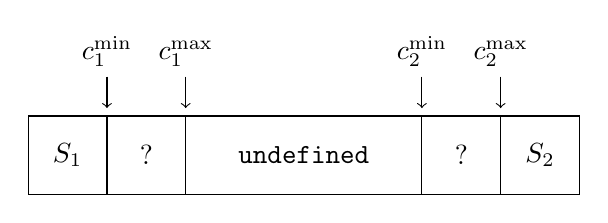
\begin{tikzpicture}
            \draw (0, 0) rectangle (1, 1) node[midway] {$S_1$};
            \draw (1, 0) rectangle (2, 1) node[midway] {$?$};
            \draw (2, 0) rectangle (5, 1) node[midway] {$\texttt{undefined}$};
            \draw (5, 0) rectangle (6, 1) node[midway] {$?$};
            \draw (6, 0) rectangle (7, 1) node[midway] {$S_2$};

            \draw[->] (1, 1.5) node[above] {$c_1^{\min}$} -- (1, 1.1);
            \draw[->] (2, 1.5) node[above] {$c_1^{\max}$} -- (2, 1.1);
            \draw[->] (5, 1.5) node[above] {$c_2^{\min}$} -- (5, 1.1);
            \draw[->] (6, 1.5) node[above] {$c_2^{\max}$} -- (6, 1.1);
        \end{tikzpicture}
    }
    \caption{The points $P$ after local partition. The points in $?$ can
             belong to either $S_1$, $S_2$, or can be undefined.}
    \label{fig:local_part}
\end{figure}

\subsubsection{Cleanup}

\tkcomment{Not yet implemented.}

In essence, the cleanup step is a Dutch National Flag Problem \cite{}: 
we have to partition into $S_1$, undefined points, $S_2$. If a point has not 
been moved, we can classify it by determining which $P^{(t)}$ its index belongs 
to, and then compare it against $c_1^{(t)}, c_2^{(t)}$. Unfortunately, the
standard algorithm proposed by Dijkstra moves some points twice, so we have
to make some modifications.

To simplify the analysis, we pretend the set we are working on is indexed
$[0, m)$.

We maintain three pointers $i \leq j < k$ and the following invariant: 
$P[0, i) \subseteq S_1$, $[i, j) \subseteq S_2$, $P[j, k)$ still have to be
sorted, $P[k, m)$ are undefined (Figure~\ref{fig:dnf}). As we can only 
classify points by comparing their index to $c_1^{(t)}, c_2^{(t)}$, we 
additionally require that inspected points have not been moved in a previous
iteration.

\begin{figure}[ht]
    \resizebox{\columnwidth}{!}{%
        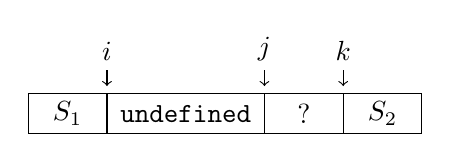
\begin{tikzpicture}
            \draw (0, 0) rectangle (1, 0.5) node[midway] {$S_1$};
            \draw (1, 0) rectangle (3, 0.5) node[midway] {$\texttt{undefined}$};
            \draw (3, 0) rectangle (4, 0.5) node[midway] {$?$};
            \draw (4, 0) rectangle (5, 0.5) node[midway] {$S_2$};

            \draw[->] (1, 0.8) node[above] {$i$} -- (1, 0.6);
            \draw[->] (3, 0.8) node[above] {$j$} -- (3, 0.6);
            \draw[->] (4, 0.8) node[above] {$k$} -- (4, 0.6);
        \end{tikzpicture}
    }
    \caption{The invariant for our Dutch National Flag variant.}
    \label{fig:dnf}
\end{figure}

\begin{algorithm}[ht]
\begin{algorithmic}[1]
    \caption{Dutch National Flag}\label{alg:dnf}
    \Require Points $P$, considered on indices $[start, end)$.
    \Ensure Permuted $P[start, end)$ and $i, j$, such that
            $P[start, i) = P[start, end) \cap S_1$ and
            $P[k, j) = P[start, end) \cap S_2$.
    \State Let $i = j = start$, $k = end$.
    \While{$j < k$}
        \If{$P[j] \in S_1$}
            \State $P[i] = P[j]$
            \State $i = i + 1$
            \State $j = j + 1$
        \ElsIf{$P[j] \notin S_1 \cup S_2$}
            \State $j = j + 1$
        \Else
            \State $k = k - 1$
            \While{$P[k] \in S_2$}
                \State $k = k - 1$
                \If{$k = j$}
                    \State \Return{}
                \EndIf
            \EndWhile
            \If{$P[k] \in S_1$}
                \State $P[i] = P[k]$
                \State $i = i + 1$
            \EndIf
            \State $P[k] = P[j]$
            \State $j = j + 1$
        \EndIf
    \EndWhile
\end{algorithmic}
\end{algorithm}

\begin{proof}
    The top-level loop will eventually terminate with $P[j, k)$ empty as 
    $j$ is incremented every iteration. 

    It is clear that the invariant is respected in the cases $P[j] \in S_1$
    and $P[j] \notin S_1 \cup S_2$.
\end{proof}

If $c_1^{\max} \leq c_2^{\min}$, we employ Algorithm~\ref{alg:dnf} with
$start = [c_1^{\min}$, $end = c_2^{\max})$, giving us 
(Figure~\ref{fig:dnf_cleanup1}). Moving $[i, j)$ up is then straightforward.

\begin{figure}[ht]
    \resizebox{\columnwidth}{!}{%
        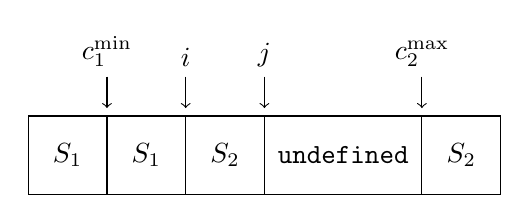
\begin{tikzpicture}
            \draw (0, 0) rectangle (1, 1) node[midway] {$S_1$};
            \draw (1, 0) rectangle (2, 1) node[midway] {$S_1$};
            \draw (2, 0) rectangle (3, 1) node[midway] {$S_2$};
            \draw (3, 0) rectangle (5, 1) node[midway] {\texttt{undefined}};
            \draw (5, 0) rectangle (6, 1) node[midway] {$S_2$};

            \draw[->] (1, 1.5) node[above] {$c_1^{\min}$} -- (1, 1.1);
            \draw[->] (2, 1.5) node[above] {$i$} -- (2, 1.1);
            \draw[->] (3, 1.5) node[above] {$j$} -- (3, 1.1);
            \draw[->] (5, 1.5) node[above] {$c_2^{\max}$} -- (5, 1.1);
        \end{tikzpicture}
    }
    \caption{The points $P$ after local partition and Dutch National Flag
             on $[c_1^{\min}, c_2^{\max})$. We then move $[i, j)$ to
             $[c_2^{\max} - (j - i), c_2^{\max})$.}
    \label{fig:dnf_cleanup1}
\end{figure}

If $c_1^{\max} > c_2^{\min}$, we employ Algorithm~\ref{alg:dnf} twice: once
on $[c_1^{\min}, c_1^{\max})$, and once on $[c_2^{\min}, c_2^{\max})$
(Figure~\ref{fig:dnf_cleanup2}). We then, ...

\begin{figure}[ht]
    \resizebox{\columnwidth}{!}{%
        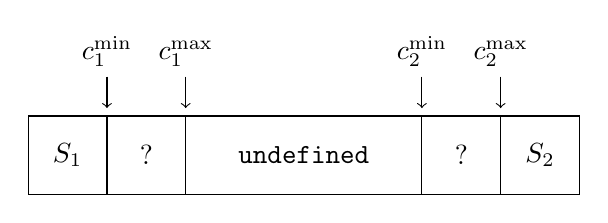
\begin{tikzpicture}
            \draw (0, 0) rectangle (1, 1) node[midway] {$S_1$};
            \draw (1, 0) rectangle (2, 1) node[midway] {$?$};
            \draw (2, 0) rectangle (5, 1) node[midway] {$\texttt{undefined}$};
            \draw (5, 0) rectangle (6, 1) node[midway] {$?$};
            \draw (6, 0) rectangle (7, 1) node[midway] {$S_2$};

            \draw[->] (1, 1.5) node[above] {$c_1^{\min}$} -- (1, 1.1);
            \draw[->] (2, 1.5) node[above] {$c_1^{\max}$} -- (2, 1.1);
            \draw[->] (5, 1.5) node[above] {$c_2^{\min}$} -- (5, 1.1);
            \draw[->] (6, 1.5) node[above] {$c_2^{\max}$} -- (6, 1.1);
        \end{tikzpicture}
    }
    \caption{The points $P$ after local partition and Dutch National Flag
             on $[c_1^{\min}, c_2^{\max})$. We then move $[i, j)$ to
             $[c_2^{\max} - (j - i), c_2^{\max})$.
             $k$ cannot be undefined, and the point under $j$ has not been 
             moved.}
    \label{fig:dnf_cleanup2}
\end{figure}

\subsubsection{Implementation Details}

\tkcomment{round down n so the reads do not cross blocks, explain how we handle
the write crossing blocks, cheap branches, false sharing, keep the index in
two integers to allow for fast checking, check whether 
$c_1^{\max} > c_2^{\min}$ etc.}
